\documentclass[
../../EiKI_Summary.tex,
]
{subfiles}
    
\externaldocument[ext:]{../../EiKI_Summary.tex}
% Set Graphics Path, so pictures load correctly
\graphicspath{{../../}}

\begin{document}
\section{Uninformed and Informed Search}
\subsection{Problem Solving}
\subsubsection{Key Terminology}

\begin{defbox}
    [State Space / States]
    A state is a possible situation in our environment - The State Space is a set of all possible states, reachable from the initial state. 
    
    Often visualized as a \defc{state-space graph} that displays all reachable states and its transitions.

    \begin{center}
        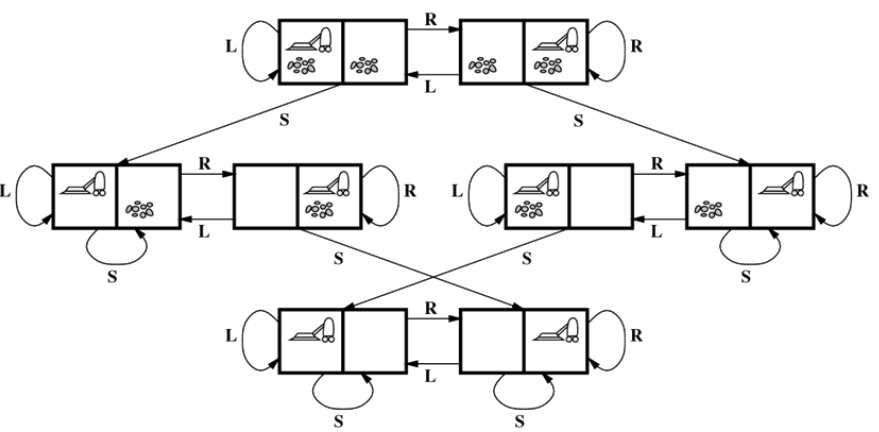
\includegraphics[width=0.6\textwidth]{Pics/03/StateSpaceGraph.png}
        \captionof{figure}{State-Space Graph of a robot vacuum cleaning}
    \end{center}
\end{defbox}

\begin{defbox}
    [Transition / Action]
    A Transition describes possible actions to take to get from one state to another. We only count direct transitions between two states (single actions)
\end{defbox}

\begin{defbox}
    [Costs]
    Transitions often differ in different qualities. We add a ''cost'' to each action, so we can rate an algorithm on how cost effective it is. 
\end{defbox}

\begin{defbox}
    [Path]
    A sequence of states connected by a sequence of actions
\end{defbox}

\begin{defbox}
    [Solution]
    A path that leads from the initial state to a goal state
\end{defbox}

\begin{defbox}
    [Optimal Solution]
    The Solution with the minimal path cost
\end{defbox}

\defc{Problem Components:}
\begin{enumerate}
    \item \defc{State Space and Initial State:} 
    \subitem All possible states and the initial environment as a state
    \item \defc{Descriptions of Actions: }
    \subitem Function that maps a state to a set of possible actions in this state
    \item \defc{Goal Test: }
    \subitem Typically a function to test if the current state fulfills the goal
    \item \defc{Costs:} 
    \subitem A cost funciton that maps actions to costs
    \subitem An easy way it to add costs of all actions taken
\end{enumerate}

Now that we have defined problems, lets go on to solutions. Most problems can be defined as \defc{planning problems}, in which we start from an initial state and transform it into a desired goal considering future actions and outcomes. 

To solve these problems we usually utilize \defc{search} algorithms to find a (optimal) solution in form of a sequence of actions.

\subsubsection{Tree Search Algorithms}
Hereby we treat the state-space graph as a tree, starting with the initial state. Using this approach we can define iterative or recursive algorithms to search for suitable paths.

\begin{codebox}
    [Example Tree Search]
    \begin{algorithm}[H]
        \SetKwFunction{trs}{tree\_search}
        \Fn{\trs{problem, strategy}}{
            initialize search tree with initial state of problem\;
            \While{\KwTrue}{
                \If{Node contains goal state}{
                    \KwRet solution
                    }
                \ElseIf{No suitable candidates for expansion}{
                    \KwRet failure
                }
                \Else{
                    Expand node and add resulting nodes to the tree
                }
            }
        }
    \end{algorithm}
\end{codebox}
\begin{minipage}
    [t]{0.45\textwidth}
    \centering
    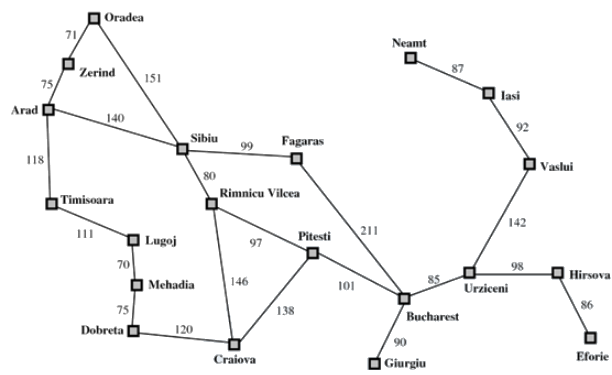
\includegraphics[width=\textwidth]{Pics/03/ExampleTreeSearchGraph.png}
\end{minipage}
\hfill
\begin{minipage}
    [t]{0.55\textwidth}
    \centering
    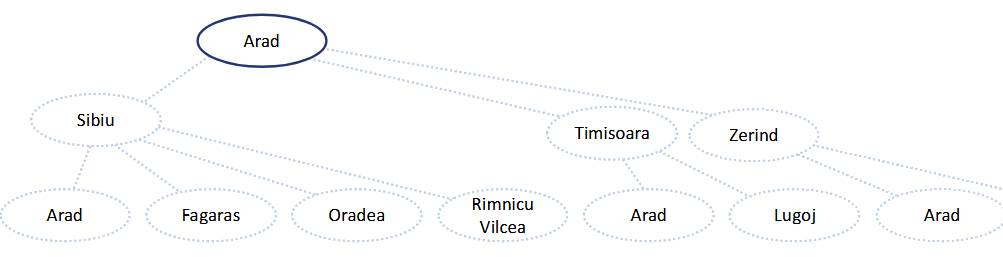
\includegraphics[width=\textwidth]{Pics/03/ExampleTreeSearchTree.png}
\end{minipage}

Each Node in the search tree is an entire path in the state-space graph. We construct both on demand - only as much as we need (won't get all solutions)

\begin{defbox}
    [Node]
    Describes a part of a tree. Includes \defc{state, parent node, taken action, path cost and depth of the tree}
\end{defbox}

\begin{defbox}
    [Fringe]
    Describes the set of nodes at the end of all visited paths
\end{defbox}

\begin{defbox}
    [Depth]
    Number of levels in the search tree
\end{defbox}

\subsection{Uninformed Search}
\begin{defbox}
    [Definition]
    The uninformed search strategy only has the problem definition, no additional information. 

    Some algorithms that utilize uninformed search are:
    \begin{itemize}
        \item Uniform-Cost Search (UCS)
        \item Breadth-First Search (BFS)
        \item Depth-First Search (DFS)
        \item Depth-Limited Search (DLS)
        \item \dots
    \end{itemize}
\end{defbox}

\subsubsection{Uniform-Cost Search (UCS)}
IN UCS each node is associated with a fixed cost, which accumulate over the path. UCS uses the lowest cumulative cost to find a path.

Only works if each step has a positive cost, as otherwise infinite loops would occur

\defc{Complexity:} $O(b^{1 + \lfloor \text{OptimalCost} / \text{eps}\rfloor})$ with $b$ being the branching factor (average number of children per node) and eps being the minimal cost for a step

\subsubsection{Breadth-First Search}
BFS is a special case of UCS, when all costs are equal. It starts at the root and goes through each node of a level before progressing to the next level. BFS stops as soon as it finds a solution, while UCS searches for the 'best' solution by lower cost.

\defc{Complexity:} $O(b^{d})$ with $b$ being the branching factor and $d$ being the depth of the search tree

\subsubsection{Depth-First Search (DFS)}
Depth-First Search starts at the root and continues on one branch until it finds a solution or failure. In case of failure it backtracks to the current parent node and continues on the next branch. 

Unlike UCS and BFS DFS is not complete; It fails if the search space is of infinite depth or has loops. 

It's also not optimal; More costly solutions may be found before less costly ones.

\defc{Complexity:} $O(b^m)$ with $b$ being the branching factor and $m$ being the maximum depth of the search tree

\begin{minipage}
    [t]{0.45\textwidth}
    \centering
    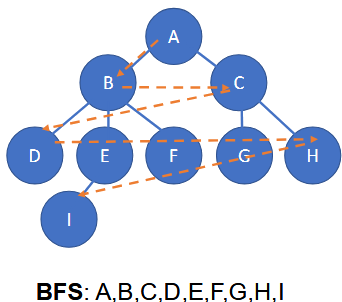
\includegraphics[width=0.9\textwidth]{Pics/03/BFSTraversal.png}
\end{minipage}
\hfill
\begin{minipage}
    [t]{0.45\textwidth}
    \centering
    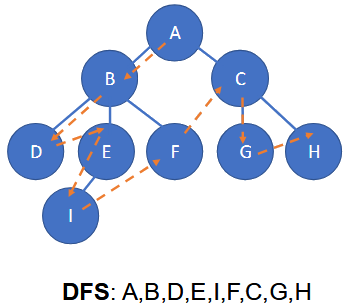
\includegraphics[width=0.9\textwidth]{Pics/03/DFSTraversal.png}
\end{minipage}

\begin{table}[h!]
    \centering
    \begin{tabular}{|>{\raggedright\arraybackslash}m{4cm}|>{\raggedright\arraybackslash}m{5cm}|>{\raggedright\arraybackslash}m{5cm}|}
    \hline
    \textbf{Criteria} & \textbf{BFS} & \textbf{DFS} \\
    \hline
    \textbf{Concept} & Traversing tree level by level & Traversing tree sub-tree by sub-tree \\
    \hline
    \textbf{Data Structure (Queue)} & First In First Out (FIFO) & Last In First Out (LIFO) \\
    \hline
    \textbf{Time Complexity} & O(Vertices + Edges) & O(Vertices + Edges) \\
    \hline
    \textbf{Backtracking} & No & Yes \\
    \hline
    \textbf{Memory} & Requires more memory & Less nodes are stored normally (less memory) \\
    \hline
    \textbf{Optimality} & Yes & Not without modification \\
    \hline
    \textbf{Speed} & In most cases slower compared to DFS & In most cases faster compared to BFS \\
    \hline
    \textbf{When to use} & If the target is relatively close to the root node & If the goal state is relatively deep in the tree \\
    \hline
    \end{tabular}
    \caption{Comparison between BFS and DFS algorithms.}
\end{table}

\newpage
\subsubsection{Depth-Limited Search (DLS)}
DLS is a variant of DFS. Hereby the search is limited to a depth of $d$. This means that no infinite search can occur, the trade-off being that it might not find all solutions.

\begin{codebox}
    [Example Depth-Limited Search]
    \begin{algorithm}[H]
        \SetKwFunction{dls}{depth\_limited\_search}
        \SetKwFunction{recdls}{recursive\_dls}
        \SetKwFunction{mnode}{make\_node}
        \SetKwFunction{inist}{initial\_state}
        \SetKwFunction{GoalTest}{goal\_test}
        \SetKwFunction{State}{state}
        \SetKwFunction{Depth}{depth}
        \SetKwFunction{Expand}{expand}
        \Fn{\dls{problem, limit}}{
            \recdls{\mnode{\inist{problem}}, problem, limit}
        }
        \Fn{\recdls{node, problem, limit}}{
            cutoff\_occured = \KwFalse\;
            \If{\GoalTest{problem, \State{node}}}{
                \KwRet node\;
            }
            \ElseIf{\Depth{node} >= limit}{
                \KwRet cutoff\;
            }
            \Else{
                \ForEach{successor in \Expand{node, problem}}{
                    result = \recdls{successor, problem, limit}\;
                    \If{result == cutoff}{
                        cutoff\_occured = \KwTrue\;
                    }
                    \ElseIf{result != failure}{
                        \KwRet result\;
                    }
                }
            }
            \If{cutoff\_occured}{
                \KwRet cutoff\;
            }
            \Else{
                \KwRet failure
            }
        }
    \end{algorithm}
\end{codebox}

This, of course, is neither complete nor optimal.

\defc{Complexity:} $O(b^l)$ with $b$ being the branching factor and $l$ being the maximum depth of the search tree

\subsubsection{Iterative Deepening Search (IDS)}
IDS is a variant of DLS. It works like DLS, but instead of a fixed depth, it iteratively increases the depth until a solution is found.

\begin{codebox}
    [Example Iterative Deepening Search]
    \begin{algorithm}[H]
        \SetKwFunction{ids}{iterative\_deepening\_search}
        \SetKwFunction{dls}{depth\_limited\_search}
        \Fn{\ids{problem}}{
            \For{depth = 0 to $\infty$}{
                result = \dls{problem, depth}\;
                \If{result != cutoff}{
                    \KwRet result
                }
            }
        }
    \end{algorithm}
\end{codebox}

This change makes it complete and optimal. 

\defc{Complexity:} $O(b^m)$ with $b$ being the branching factor and $d$ being the depth of the search tree. This makes its time complexity equal to BFS. However, the space complexity of IDS is $O(bd)$, which is much better than BFS' $O(b^d)$.

\begin{table}[h!]
    \centering
    \begin{tabular}{@{}lccccc@{}}
    \toprule
    Criterion          & Breadth-First & Uniform-Cost & Depth-First & Depth-Limited & Iterative Deepening \\ \midrule
    Complete?          & Yes$^*$       & Yes$^*$      & No          & Yes, if $l \geq d$ & Yes                 \\
    Time               & $b^{d}$     & $b^{1 + \lfloor OptCost / eps \rfloor}$ & $b^m$       & $b^l$          & $b^d$              \\
    Space              & $b^{d}$     & $b^{1 + \lfloor OptCost / eps \rfloor}$ & $bm$        & $bl$           & $bd$               \\
    Optimal?           & Yes$^*$       & Yes          & No          & No            & Yes$^*$          \\ \bottomrule
    \end{tabular}
    \caption{Comparison of search strategies.}
\end{table}

\newpage
\subsection{Heuristics h}
\begin{defbox*}
    Denotes a ''rule of thumb'', a rule that may be helpful in solving a problem.

    In Tree-Search, a heuristic is a function that estimates the remaining cost from the current node to the goal.

    \defc{Can go wrong!}
\end{defbox*}

\begin{defbox}
    [Admissible Heuristic]
    A heuristic is admissible if it never overestimates the actual cost to reach the goal.
    
    \begin{center}
        \inlmathbox{$h(n) \leq h^*(n)$}\\
        if $h^*(n)$ is the true cost to reach the goal from node $n$
    \end{center}
\end{defbox}

\begin{defbox}
    [Consistent Heuristic]
    A heuristic is consistent if for every node $n$ and successor $n'$ generated by any action $a$: 
    \begin{center}
        \inlmathbox{$h(n) \leq c(n, a, n') + h(n')$}\\
        if $c(n, a, n')$ is the cost of the action $a$ from $n$ to $n'$
    \end{center}
    Thus, a heuristic is consistent if, when going from neighboring nodes, the heuristic difference / step cost never overestimates the actual cost.
\end{defbox}

\begin{defbox}
    [Lemmas]
    \begin{itemize}
        \item If a heuristic is consistent, it is also admissible.
        \item If $h(n)$ is consistent, then the values of $f(n)$ on any path are non-decreasing.
    \end{itemize}
\end{defbox}

\subsubsection{Relaxed Problems}
\begin{defbox*}
    A relaxed problem is a problem that has fewer constraints on the actions than the original problem.
\end{defbox*}

The cost of the optimal solution to a relaxed problem is an admissible heuristic for the original problem.

\defc{Example:} Relaxed Problem as Admissible Heuristic\\
    Consider a grid-based pathfinding problem where certain movements are restricted due to obstacles. A relaxed version of this problem might allow movement through obstacles by ignoring some constraints. The cost of the optimal solution to this relaxed problem, which is typically lower or equal to the original problem's optimal cost, serves as an admissible heuristic for the original problem.

This means that looking for relaxed problems is a good way to find admissible heuristics.

\subsubsection{Dominance}
\begin{defbox*}
    A heuristic $h_2$ dominates $h_1$ if $h_2(n) \geq h_1(n)$ for all nodes $n$. (Given that $h_1$ and $h_2$ are admissible)
\end{defbox*}

This means that a dominant heuristic is always closer to the optimal heuristic h*, which results in less expansion and thus more efficient search.

\subsubsection{Combining Heuristics}
\begin{defbox*}
    If $h_1$, $h_2$, \dots $h_m$ are admissible heuristics, then $h(n) = max(h_1(n), h_2(n),\dots,  h_m(n))$ is also admissible and dominates both $h_1$ and $h_2$.
\end{defbox*}

This is useful if we have multiple admissible non-dominated heuristics and want to combine them to get a better heuristic. 

\subsection{Informed Search}
\begin{defbox}
    [Definition]
    The informed search strategy has additional knowledge about ''where'' to look for solutions, usually in form of a heuristic function.

    Some algorithms that utilize informed search are:
    \begin{itemize}
        \item Greedy Best-First Search
        \item A* Search
        \item Memory-Bounded Heuristic Search
    \end{itemize}
\end{defbox}


\subsubsection{Greedy Best-First Search}
Greedy Best-First Search (GBFS) is an informed search algorithm that selects the next node to expand based on a heuristic that estimates the cost from the current node to the goal. 

One example of a heuristic is the straight-line distance to the goal. 

\begin{figure}[h!]
    \centering
    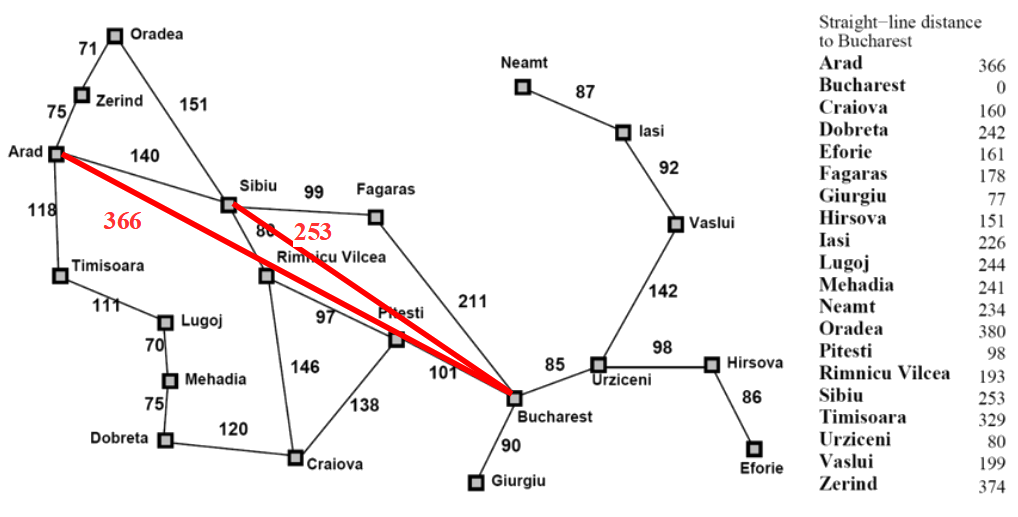
\includegraphics[width=0.6\textwidth]{Pics/03/GreedyBestFirstExample.png}
    \caption{Example of GBFS with a straight-line distance heuristic.}
\end{figure}

\defc{Complexity:} The time complexity of Greedy Best-First Search is $O(b^m)$, and its space complexity is also $O(b^m)$, where $b$ is the branching factor and $m$ is the maximum depth of the search tree. This is the same as DFS, however due to the heuristic it can be significantly faster.

GBFS is not guaranteed to be optimal or complete, especially if the heuristic function is not admissible or consistent. Its efficiency heavily depends on the quality of the heuristic used.

\begin{itemize}
    \item \textbf{Complete?} No, can get stuck in loops.
    \item \textbf{Optimal?} No, does not guarantee an optimal solution as it depends on the heuristic, which may be flawed.
\end{itemize}


\subsubsection{A* Search}
\begin{defbox}
    [Definition]
    A* Search is an informed search algorithm that combines the strengths of Uniform-Cost Search and Greedy Best-First Search. It searches for the least-cost path to the goal by considering both the cost to reach the current node and an estimated cost to reach the goal.
\end{defbox}

A* Search tries to avoid paths that are already expensive. It evaluates the complete path cost and the remaining cost to the goal. Its cost function is defined as $f(n) = g(n) + h(n)$, where $g(n)$ is the cost to reach the current node (root to n) and $h(n)$ (the heuristic) is the estimated cost to reach the goal (n to goal).

\begin{figure}[htp]
    \centering
    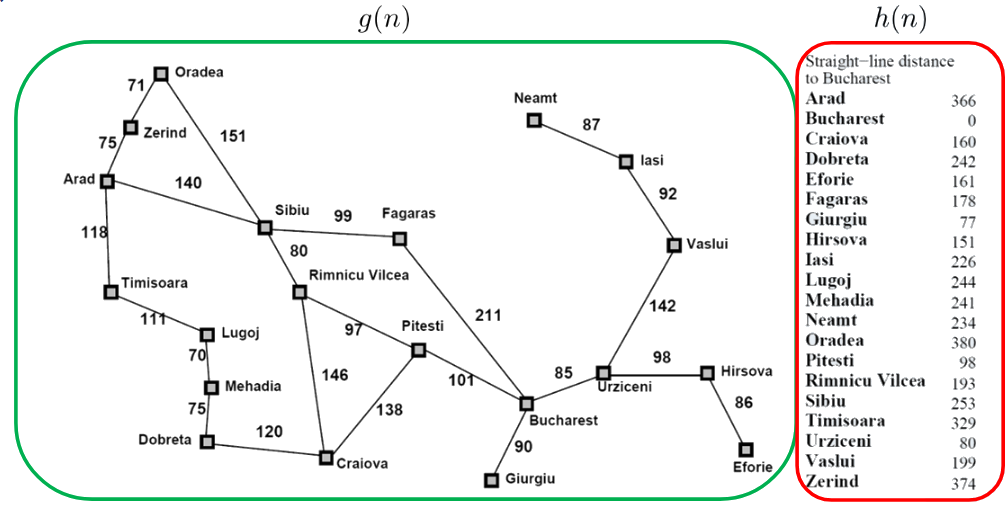
\includegraphics[width=0.6\textwidth]{Pics/03/AStarSearchExample.png}
    \caption{Example of A* Search with heuristic function.}
\end{figure}

\defc{Complexity:} The time complexity of A* Search is $O(b^m)$, and its space complexity is also $O(b^m)$, where $b$ is the branching factor and $m$ is the maximum depth of the search tree.

\defc{Completeness and Optimality:} A* Search is complete, and can be optimal, if the heuristic is admissible.

\subsubsection{Alternatives to A*}
\begin{enumerate}
    \item \defc{Iterative-Deepening A* (IDA*)}
    \begin{itemize}
        \item Like iterative deepening, it explores nodes level by level, but uses A* to evaluate the nodes.
        \item Cutoff information is the f-cost (g + h) instead of the depth.
    \end{itemize}
    \item \defc{Recursive Best-First Search (RBFS)}
    \begin{itemize}
        \item Recursive algorithm that mimics best-first search with linear space
        \item Keeps track of f-value of best alternative path
        \item Path available from any ancestor of the current node and heuristic evaluations are updated with results of successors
    \end{itemize}
    \item \defc{(Simple) Memory-Bounded A* ((S)MA*)}
    \begin{itemize}
        \item Drops the worst leaf node when memory is full
        \item Its value will be updated to its parent
        \item May be researched later
    \end{itemize}
\end{enumerate}

\subsubsection{Graph Search}
When traversing a problem, loops can occur. Failure to detect them can turn linear search into exponential search.
To avoid this, we can use \defc{graph search}. Hereby we only expand nodes that have not been visited yet.

For example: The graph search version of UCS is \defc{Dijkstra's algorithm}.
\end{document}